\documentclass[tikz,border=5mm]{standalone}
\usepackage{tikz}
\usetikzlibrary{positioning, shapes.geometric}

\definecolor{graybg}{RGB}{217,217,217}

\tikzset{
    every node/.style={
        font=\sffamily,
        align=center
    },
    box/.style={
        rectangle,
        fill=graybg,
        draw=black,
        minimum width=1.5cm,
        minimum height=1cm,
        rounded corners=2pt,
        outer sep=0pt
    },
    circle/.style={
        ellipse,
        fill=graybg,
        draw=black,
        minimum width=1.5cm,
        minimum height=1cm,
        outer sep=0pt
    },
    dashedbox/.style={
        box,
        dash pattern=on 2pt off 2pt,
        draw=gray
    },
    arrow/.style={
        ->,
        >=latex,
        thick,
        black
    },
    dashedarrow/.style={
        arrow,
        dashed,
        dash pattern=on 2pt off 2pt,
        draw=gray
    },
    dottedarrow/.style={
        arrow,
        densely dotted,
        draw=gray
    },
}

\begin{document}
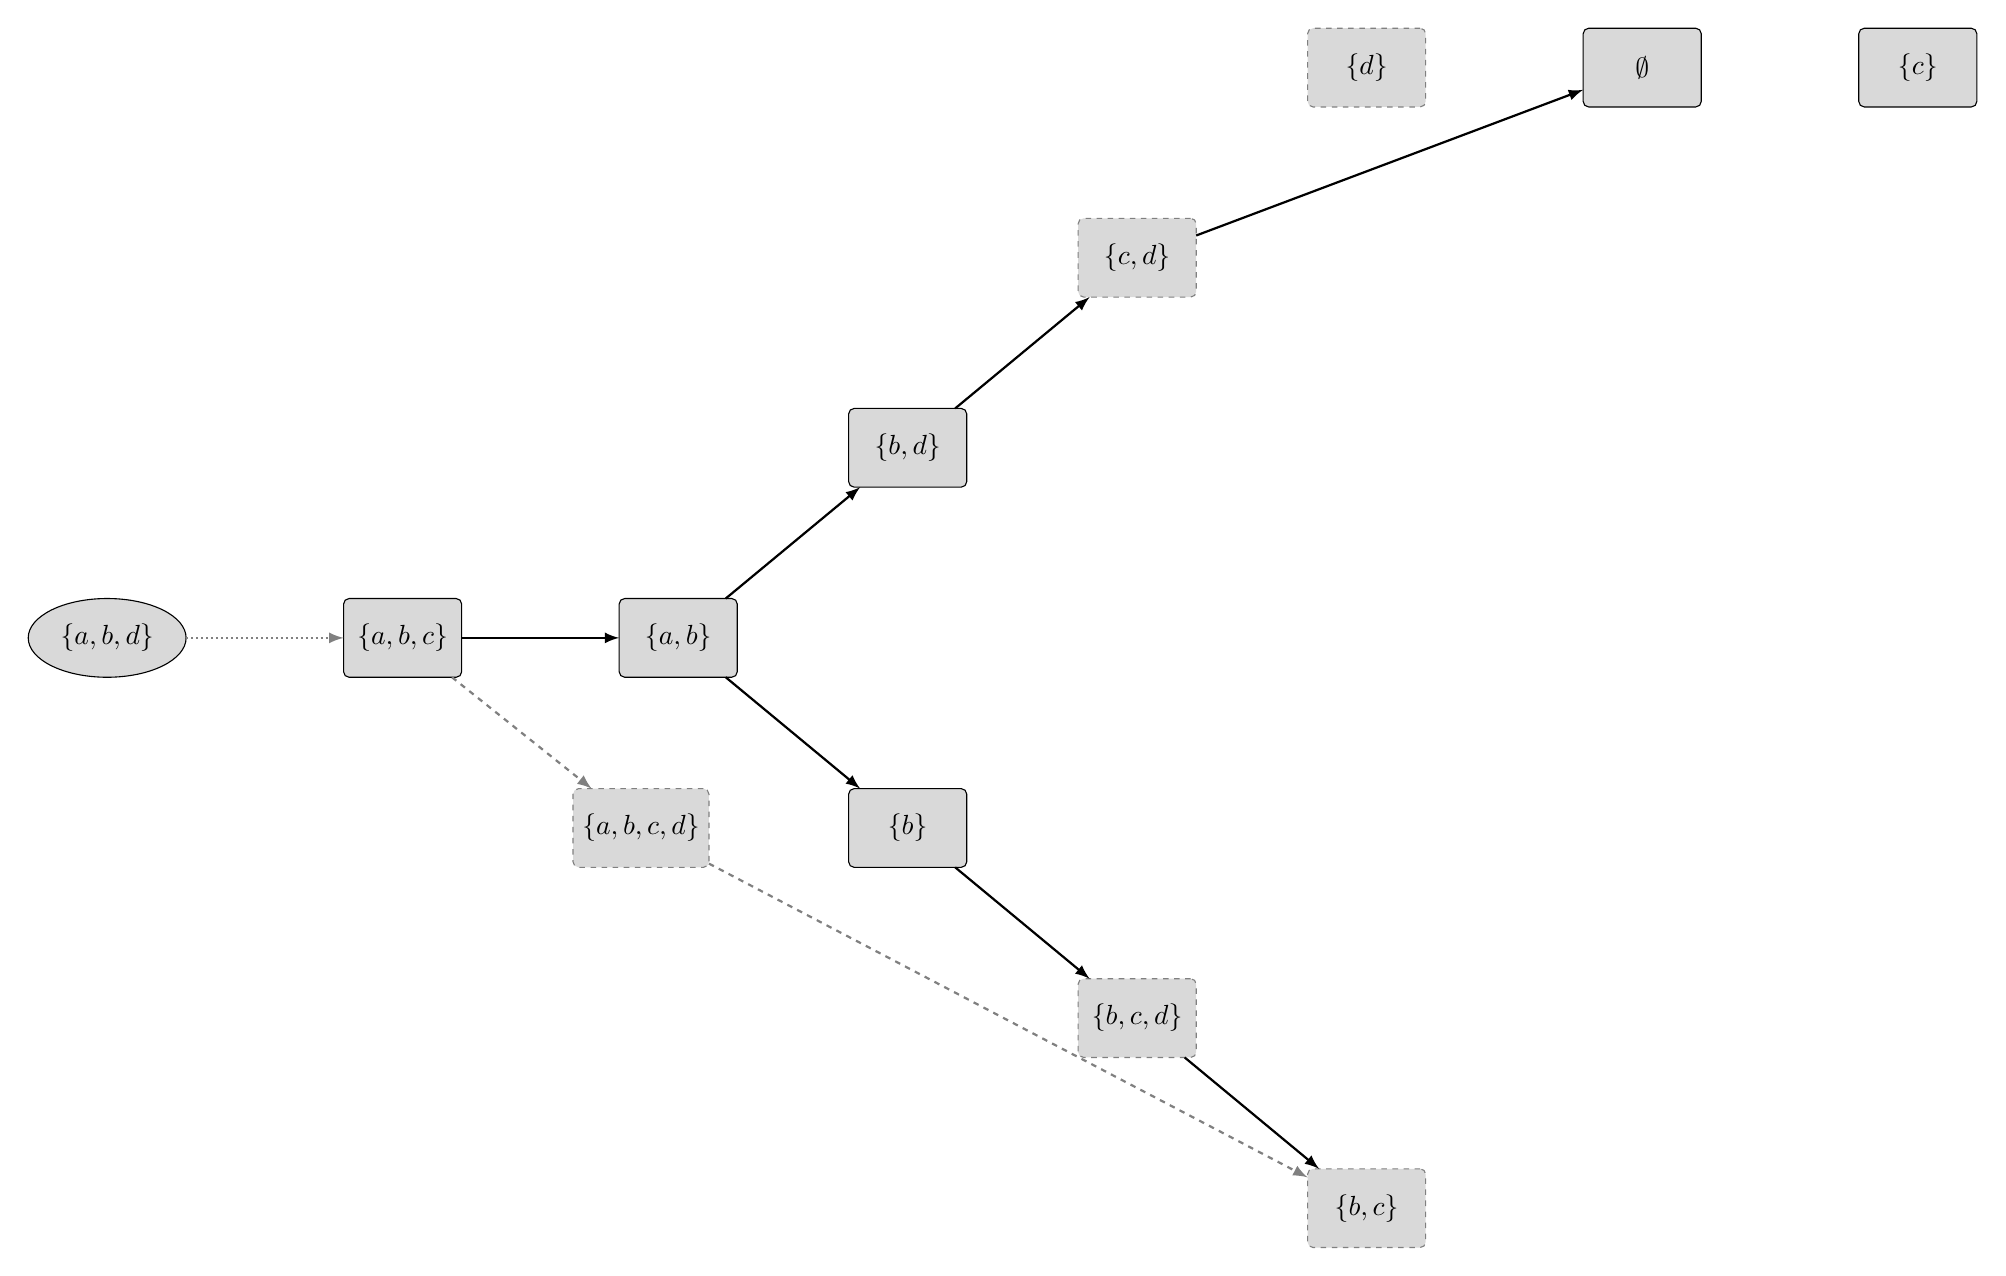
\begin{tikzpicture}[node distance=2cm]

    % Leftmost nodes
    \node[circle] (c1) at (-6,0) {$\{a,b,d\}$};
    \node[box, right=of c1] (b1) {$\{a,b,c\}$};
    \node[box, right=of b1] (b2) {$\{a,b\}$};
    
    % Middle nodes
    \node[box, above right=of b2] (b3) {$\{b,d\}$};
    \node[box, below right=of b2] (b4) {$\{b\}$};
    
    % Rightmost nodes
    \node[dashedbox, above right=of b3] (b5) {$\{c,d\}$};
    \node[dashedbox, below right=of b4] (b6) {$\{b,c,d\}$};
    \node[dashedbox, below right=of b1] (b7) {$\{a,b,c,d\}$};
    \node[dashedbox, above right=of b5] (b8) {$\{d\}$};
    \node[dashedbox, below right=of b6] (b9) {$\{b,c\}$};
    
    % Top-right nodes
    \node[box, right=of b8] (b10) {$\emptyset$};
    \node[box, right=of b10] (b11) {$\{c\}$};
    
    % Arrows
    \draw[dottedarrow] (c1) -- (b1);
    \draw[arrow] (b1) -- (b2);
    \draw[arrow] (b2) -- (b3);
    \draw[arrow] (b2) -- (b4);
    \draw[arrow] (b3) -- (b5);
    \draw[arrow] (b4) -- (b6);
    \draw[arrow] (b5) -- (b10);
    \draw[arrow] (b6) -- (b9);
    \draw[dashedarrow] (b1) -- (b7);
    \draw[dashedarrow] (b7) -- (b9);

\end{tikzpicture}
\end{document}